\documentclass[17pt,ignorenonframetext,]{beamer}
\usefonttheme{structurebold}
\setbeamertemplate{caption}[numbered]
\setbeamertemplate{caption label separator}{:}
\setbeamercolor{caption name}{fg=normal text.fg}
\usepackage{amssymb,amsmath}
\usepackage{ifxetex,ifluatex}
\usepackage{fixltx2e} % provides \textsubscript
\usepackage{lmodern}
\ifxetex
  \usepackage{fontspec,xltxtra,xunicode}
  \defaultfontfeatures{Mapping=tex-text,Scale=MatchLowercase}
  \newcommand{\euro}{€}
\else
  \ifluatex
    \usepackage{fontspec}
    \defaultfontfeatures{Mapping=tex-text,Scale=MatchLowercase}
    \newcommand{\euro}{€}
  \else
    \usepackage[T1]{fontenc}
    \usepackage[utf8]{inputenc}
      \fi
\fi
% use upquote if available, for straight quotes in verbatim environments
\IfFileExists{upquote.sty}{\usepackage{upquote}}{}
% use microtype if available
\IfFileExists{microtype.sty}{\usepackage{microtype}}{}
\usepackage{graphicx}
\makeatletter
\def\maxwidth{\ifdim\Gin@nat@width>\linewidth\linewidth\else\Gin@nat@width\fi}
\def\maxheight{\ifdim\Gin@nat@height>\textheight0.8\textheight\else\Gin@nat@height\fi}
\makeatother
% Scale images if necessary, so that they will not overflow the page
% margins by default, and it is still possible to overwrite the defaults
% using explicit options in \includegraphics[width, height, ...]{}
\setkeys{Gin}{width=\maxwidth,height=\maxheight,keepaspectratio}

% Comment these out if you don't want a slide with just the
% part/section/subsection/subsubsection title:
\AtBeginPart{
  \let\insertpartnumber\relax
  \let\partname\relax
  \frame{\partpage}
}
\AtBeginSection{
  \let\insertsectionnumber\relax
  \let\sectionname\relax
  \frame{\sectionpage}
}
\AtBeginSubsection{
  \let\insertsubsectionnumber\relax
  \let\subsectionname\relax
  \frame{\subsectionpage}
}

\usepackage[normalem]{ulem}
% avoid problems with \sout in headers with hyperref:
\pdfstringdefDisableCommands{\renewcommand{\sout}{}}
\setlength{\parindent}{0pt}
\setlength{\parskip}{6pt plus 2pt minus 1pt}
\setlength{\emergencystretch}{3em}  % prevent overfull lines
\setcounter{secnumdepth}{0}
\definecolor{Black1}{RGB}{43,40,40}
\definecolor{Blue1}{RGB}{48, 122, 190}
\definecolor{Blue2}{RGB}{99, 151, 205}
\definecolor{Orange1}{HTML}{F5996F}
\definecolor{White1}{RGB}{255,255,243}
\definecolor{Grey1}{RGB}{164, 173, 185}
\usepackage{zxjatype}
\setjamainfont{Hiragino Kaku Gothic Pro}
\setbeamertemplate{navigation symbols}{}
\hypersetup{colorlinks = true, linkcolor = blue, citecolor = red, urlcolor = Black1}
\usepackage{fontspec}
\usepackage{fontawesome}
\setbeamerfont{title}{size = \fontsize{38}{10}}
\setbeamercolor{title}{fg = Blue1}
\setbeamerfont{subtitle}{size = \large}
\setbeamercolor{subtitle}{fg = Blue2}
\setbeamercolor{author}{fg = Black1}
\setbeamercolor{normal text}{fg = Black1}
\setbeamerfont{date}{series = \itshape}
\setbeamercolor{date}{fg = Grey1}
\setbeamercolor{frametitle}{fg = Blue1}
\setbeamercolor{section in toc}{fg = Grey1}

\title{前処理のための前処理}
\subtitle{シリーズ前処理2015}
\author{@u\_ribo}
\date{Tokyo.R\#45 January 17, 2015}

\begin{document}
\frame{\titlepage}

\begin{frame}

\center{
  \Huge{\textbf{\textcolor{magenta}{Tokyo.R} \\シリーズ前処理: \\おさらい}}
}

\end{frame}

\begin{frame}{\faFood 前処理}

\center{
  \LARGE{【広義】手元にある観測データを、意図する分析手法が適用できる形にまでもっていく方法}
}

\begin{quote}
\scriptsize{\faLink http://www.slideshare.net/dichika/maeshori-missing}
\end{quote}

\end{frame}

\begin{frame}{\faFood 前処理}

\includegraphics{images/work_time_ratio-1.pdf}

\scriptsize{\faBook Dasu and Johnson 2003. Exploratory Data Mining and Data Cleaning. \textit{Wiley}}

\end{frame}

\begin{frame}{\faFood 前処理}

\center{
  \Huge{\faTime 解析時間の\\ほとんどは前処理}
}

\end{frame}

\begin{frame}

{[}1{]} ``ムダ'' ``ムダ'' ``ムダ'' {[}4{]} ``ムダ'' ``ムダ'' ``ムダ''
{[}7{]} ``ムダ'' ``ムダ'' ``ムダ'' {[}10{]} ``ムダ'' ``ムダ'' ``ムダ''
{[}13{]} ``ムダ'' ``ムダ'' ``ムダ'' {[}16{]} ``ムダ'' ``ムダ'' ``ムダ''
{[}19{]} ``ムダ'' ``ムダ'' ``ムダ'' {[}22{]} ``ムダ'' ``ムダ'' ``ムダ''
{[}25{]} ``ムダ'' ``ムダ'' ``ムダ'' {[}28{]} ``ムダ'' ``ムダ'' ``ムダ''
{[}31{]} ``ムダ'' ``ムダ'' ``ムダ'' {[}34{]} ``ムダ'' ``ムダ'' ``ムダ''
{[}37{]} ``ムダ'' ``ムダ'' ``ムダ'' {[}40{]} ``ムダ'' ``ムダ'' ``ムダ''
{[}43{]} ``ムダ'' ``ムダ'' ``ムダ'' {[}46{]} ``ムダ'' ``ムダ'' ``ムダ''
{[}49{]} ``ムダ'' ``ムダ'' ``ムダ'' {[}52{]} ``ムダ'' ``ムダ'' ``ムダ''
{[}55{]} ``ムダ'' ``ムダ'' ``ムダ'' {[}58{]} ``ムダ'' ``ムダ'' ``ムダ''
{[}61{]} ``ムダ'' ``ムダ'' ``ムダ'' {[}64{]} ``ムダ'' ``ムダ'' ``ムダ''
{[}67{]} ``ムダ'' ``ムダ'' ``ムダ'' {[}70{]} ``ムダ'' ``ムダ'' ``ムダ''
{[}73{]} ``ムダ'' ``ムダ'' ``ムダ'' {[}76{]} ``ムダ'' ``ムダ'' ``ムダ''
{[}79{]} ``ムダ'' ``ムダ'' ``ムダ'' {[}82{]} ``ムダ'' ``ムダ'' ``ムダ''
{[}85{]} ``ムダ'' ``ムダ'' ``ムダ'' {[}88{]} ``ムダ'' ``ムダ'' ``ムダ''
{[}91{]} ``ムダ'' ``ムダ'' ``ムダ'' {[}94{]} ``ムダ'' ``ムダ'' ``ムダ''
{[}97{]} ``ムダ'' ``ムダ'' ``ムダ'' {[}100{]} ``ムダ''

\end{frame}

\begin{frame}

\center{
  \fontsize{120}{10}{\faThumbsDown \faThumbsDown \faThumbsDown}
}

\end{frame}

\begin{frame}

\center{
  \large{(データ処理が楽に終ることで得られる)\\\textcolor{magenta}{幸せ}について\\本気だして考えてみた}
}

\end{frame}

\begin{frame}

\center{
  \Huge{\textbf{今日のテーマ: \\\textcolor{Blue1}{前}処理のための\\\textcolor{magenta}{前}処理}}
}

\end{frame}

\begin{frame}{\large{もちべーしょん: 前処理の苦労を減らしたい}}

\begin{itemize}
\itemsep1pt\parskip0pt\parsep0pt
\item
  データ解析や前処理をする際の用意、心がけ
\item
  ぼくのがんがえた\sout{さいきょうの}こうりつてきな\textbf{まえしょり}にひつような\textbf{まえしょり}
\end{itemize}

\end{frame}

\begin{frame}{良い前処理を実現するための5箇条}

\begin{enumerate}
\def\labelenumi{\arabic{enumi}.}
\itemsep1pt\parskip0pt\parsep0pt
\item
  RStudio内ですべて完結
\item
  \texttt{.Rproj}を作成する
\item
  GitやSubversionによるバージョン管理をおこなう
\item
  \texttt{.Rmd}でファイルを保存する
\item
  プロジェクトのガイドラインを策定する
\end{enumerate}

\end{frame}

\begin{frame}

\center{
  \large{「いろいろと\textcolor{Blue2}{面倒}だ」}
  
  \huge{「でもあなたのちっぽけな\textbf{\textcolor{magenta}{頭では忘れてしまう}}でしょう(煽り)」}\
  
  \small{「ぐぬぬ」}
}

\end{frame}

\begin{frame}{何が目的か}

数時間ですべての作業が完了するプロジェクトはほとんどなく、多くのプロジェクトが長い時間を経て完成される。また、完成されてからも定期・不定記に管理する必要が生じる。そのため、プロジェクトは変動しつづけるものである。

-\textgreater{} 記録として残すことが大事

\end{frame}

\begin{frame}{dd}

\begin{itemize}
\itemsep1pt\parskip0pt\parsep0pt
\item
  以下の項目を円滑に進める体制が整っている
\item
  オープンなプロジェクトであればGitHubにリポジトリを作成する
\item
  し、コードとコメントの分離に努める
\item
  し、プロジェクト内での混乱、衝突を防ぐ
\end{itemize}

\end{frame}

\begin{frame}{Packrat\ldots{}}

\end{frame}

\begin{frame}{@dichika進捗どうですか\faEyeOpen}

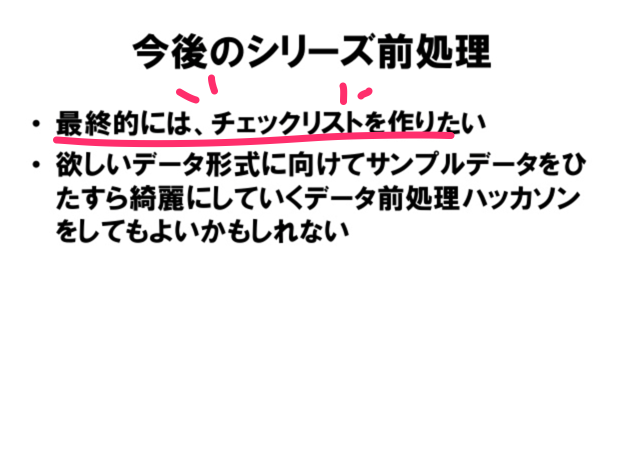
\includegraphics[angle = -3]{images/at_dichika.png}

\end{frame}

\begin{frame}{\large{Remember \textit{\textcolor{Black1}{why are you using SJIS}}}}

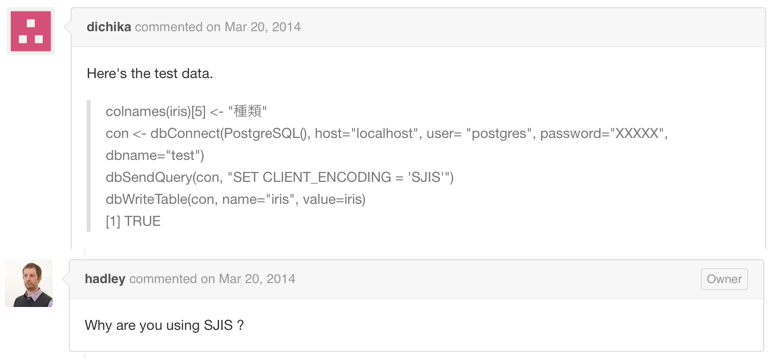
\includegraphics{images/why_are_u_using_sjis.png}

\begin{quote}
\scriptsize{\faLink https://github.com/hadley/dplyr/issues/339}
\end{quote}

\end{frame}

\begin{frame}{\#Tsurami}


\includegraphics{images/tsurami.png}

\begin{quote}
\scriptsize{\faLink https://twitter.com/yamano357/status/552514988137783301}
\end{quote}

\end{frame}

\begin{frame}{\#Tsurami}


\includegraphics{images/tsurami2.png}

\begin{quote}
\scriptsize{\faLink https://twitter.com/gg$\_$hatano/status/551328451068588032}
\end{quote}

\end{frame}

\begin{frame}{\#Tsurami}

\center{
  \Huge{供養しましょう}
  \small{\url{https://github.com/uribo/data_treatment}}
}

\end{frame}

\begin{frame}{前処理のための前処理チェックリスト}

\end{frame}

\begin{frame}{Abstract}

元データの単位変換や新たな値を算出するといった前処理の作業は、データ解析の大部分を占める作業である。一方で前処理の作業は、データを整形する、項目名を修正する、新たな項目を追加するというように、決まったパターンであることが多いため、Rによる自動的な処理が可能である。本発表では実際のデータ解析前処理において、多くの作業時間を費やすことになりがちな前処理を効率的に行うためのツールや前段階として用意しておくとよいと考えられる項目を紹介する。

\end{frame}

\begin{frame}[fragile]{\small{Sessioninfo: R version 3.1.2 (2014-10-31)}}

\begin{verbatim}
 [1] "DiagrammeR"   
 [2] "ggthemr"      
 [3] "knitcitations"
 [4] "fortunes"     
 [5] "xtable"       
 [6] "rmarkdown"    
 [7] "devtools"     
 [8] "popbio"       
 [9] "quadprog"     
[10] "ggplot2"      
[11] "glmmML"       
[12] "dplyr"        
[13] "magrittr"     
[14] "MASS"         
[15] "lattice"      
[16] "stringr"      
[17] "knitr"        
\end{verbatim}

\end{frame}

\end{document}
